\documentclass{memad-deliverable}

\usepackage{lipsum}

%\acronym{MeMAD}
%\shorttitle{Methods for Managing Audiovisual Data}
%\longtitle{Methods for Managing Audiovisual Data:\newline Combining Automatic Efficiency with\newline Human Accuracy}

%\fundingscheme{H2020-ICT-2016-2017/H2020-ICT-2017-1}
%\grantno{780069}

%\projversiondate{3.10.2017}
%\projstartdate{1.1.2018}

%\reprname{Prof. Mikko Kurimo}
%\repraffil{AALTO–KORKEAKOULUSÄÄTIÖ, Aalto University School of Electrical Engineering,\linebreak Department of Signal Processing and Acoustics}
%\repremail{mikko.kurimo@aalto.fi}

\title{MeMAD Deliverable}

\deliverableno{\#.\#}
\deliverablename{[Add deliverable name]}

\beneficiary{Add lead beneficiary}
\disseminationlevel{Add dissemination level}

\duedate{Add date}
\submissiondate{Project manager will fill in}

\author{Author 1 & Beneficiary 1 & x@y.z \\\hline
         Author 2 & Beneficiary 2 & x@y.z \\\hline
         Author 3 & Beneficiary 3 & x@y.z}

\abstract{
    \lipsum[1]
}

\begin{document}

\titlepages

\tableofcontents\clearpage

\section{Introduction}
\label{sec:intro}

\lipsum[2-8]

\begin{figure}
    \centering
    \resizebox{.8\textwidth}{!}{
        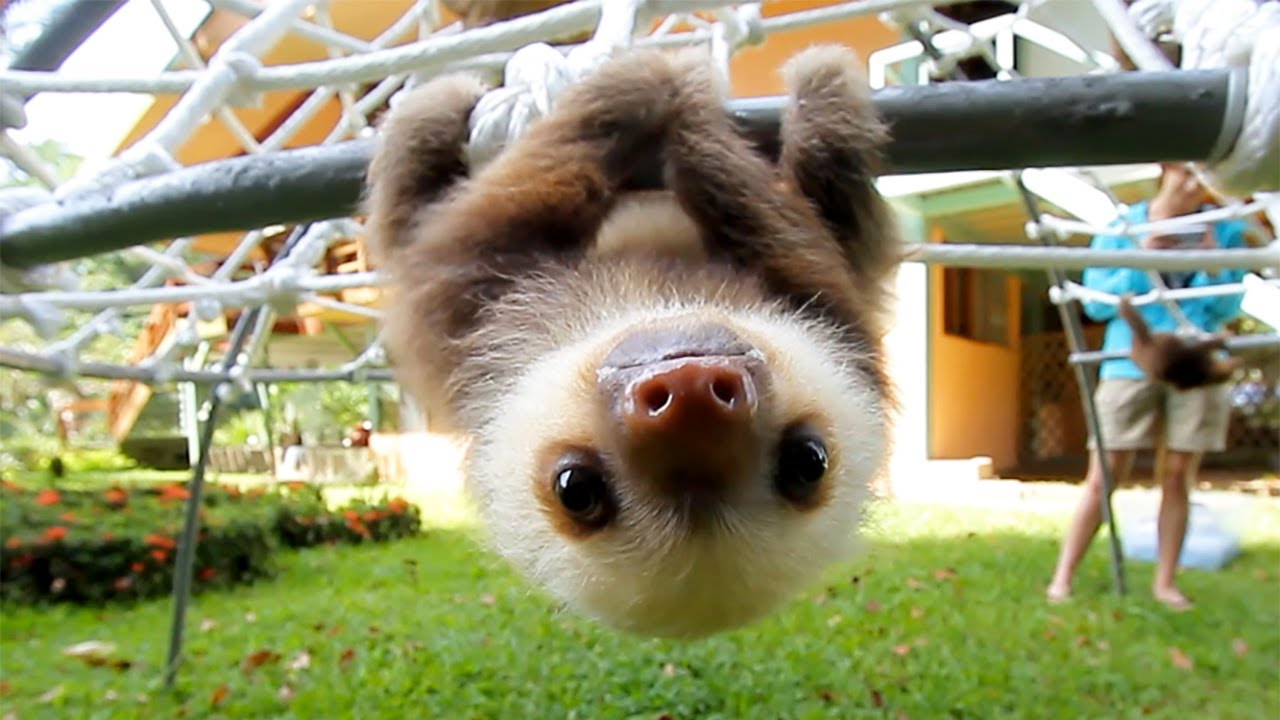
\includegraphics{example}
    }
    \caption{A baby sloth.}
    \label{fig:intro:example}
\end{figure}

\lipsum[9-14]

\section{Section}
\label{sec:sec1}

\lipsum[15-16]

\subsection{Subsection}
\label{ssec:sec1:ssec1}

\lipsum[17-18]

\subsection{Subsection}
\label{sssec:sec1:ssec2}

\lipsum[19-20]

\subsection{Subsection}
\label{sssec:sec1:ssec3}

\lipsum[21-22]

\end{document}
